%=============================================================================
% SECTION 5: GRAVITATIONAL WAVES
% Part II: Contact with Known Physics
% Equations: (23)-(34)
% Estimated pages: 10-12
%=============================================================================

\section{Gravitational Waves}\label{sec:gw}

Gravitational wave astronomy provides stringent tests of gravity in the strong-field, dynamical regime. The direct detection of binary black hole and neutron star mergers by LIGO, Virgo, and KAGRA has opened a new window for testing alternative theories. This section demonstrates that DFD reproduces GR's gravitational wave predictions at leading order, satisfying all current observational constraints while providing a framework for quantifying potential deviations through the parameterized post-Einsteinian (ppE) formalism.

%-----------------------------------------------------------------------------
\subsection{Two Gravitational Sectors on Flat $\mathbb{R}^3$}\label{sec:gw-twosector}
%-----------------------------------------------------------------------------

Before presenting the technical details, we establish the conceptual framework for gravitational radiation in DFD. This framework preserves DFD's core identity---flat Euclidean space $\mathbb{R}^3$ with absolute time $t$---while accounting for the observed tensor polarization structure of gravitational waves.

\subsubsection{The Optical Sector (DFD Core)}

DFD posits a scalar field $\psi(\mathbf{x},t)$ on flat $\mathbb{R}^3$ with absolute time $t$. The optical sector defines a refractive index $n = e^{\psi}$ and an effective optical interval:
\begin{equation}\label{eq:optical-interval}
d\tilde{s}^2 = -\frac{c^2}{n^2}dt^2 + d\mathbf{x}^2.
\end{equation}
We introduce $d\tilde{s}^2$ as a compact encoding of how $\psi$ rescales local clock rates; \textit{it is not a dynamical spacetime geometry and no curvature field equations are assumed}. The fundamental arena remains $(\mathbb{R}^3, t)$.

Local observers in regions with different $\psi$ compare clock rates by $dt_{\rm phys} = dt/n$. In DFD, $n = e^\psi$ rescales clock rates; it does not introduce an asymptotic subluminal EM signal speed relative to the shared far-zone cone. Observable light-bending and gravitational time delay are encoded via an effective travel-time functional (Fermat principle) built from $dt_{\rm phys} = dt/n$; this is used as a bookkeeping device for clock-rate comparisons and Fermat/eikonal propagation, not as a dynamical metric with curvature equations.

\subsubsection{The Radiative Sector (Tidal Disturbances)}

Compact-binary mergers exhibit gravitational radiation with \textbf{two tensor polarizations}. A scalar field $\psi$ alone cannot reproduce this polarization structure. DFD therefore distinguishes two gravitational phenomena on the same flat arena:
\begin{itemize}
\item \textbf{Optical gravity} ($\psi$): scalar field governing clock rates, refractive bending, and quasi-static matter dynamics
\item \textbf{Radiative gravity} ($h_{ij}^{\rm TT}$): transverse-traceless tensor field describing propagating tidal disturbances
\end{itemize}

The TT field is defined on $\mathbb{R}^3$ by the standard conditions:
\begin{equation}
\partial_i h_{ij}^{\rm TT} = 0, \qquad \delta^{ij}h_{ij}^{\rm TT} = 0,
\end{equation}
and obeys a wave equation on the flat background:
\begin{equation}\label{eq:TT-wave-eq}
\left(\frac{1}{c^2}\partial_t^2 - \nabla^2\right)h_{ij}^{\rm TT} = \frac{16\pi G}{c^4}\Pi_{ij}^{\rm TT},
\end{equation}
where $\Pi_{ij}^{\rm TT}$ is the TT projection of the source stress.

This is not an appeal to curved spacetime: both $\psi$ and $h_{ij}^{\rm TT}$ are fields on the same flat $(\mathbb{R}^3, t)$ arena. The radiative sector is the \textit{lowest-order consistent completion} representing the observed polarization content of gravitational waves.

\textbf{Firewall:} The radiative sector is introduced to account for observed tensor polarizations; it does not alter the optical-sector derivations of lensing, clocks, or MOND phenomenology.

We state plainly: the TT sector is not independently \textit{derived} from the scalar $\psi$-field dynamics alone.  However, both sectors emerge naturally as irreducible components of a single parent strain field on flat space, and the absence of derivative mixing between them is a structural consequence of rotational symmetry, not an ad hoc postulate.

\subsubsection{Parent Strain Field and Irreducible Decomposition}\label{sec:gw-parent}

Define a symmetric strain field on flat $\mathbb{R}^3$:
\begin{equation}\label{eq:parent-strain}
\Psi_{ij} = \frac{1}{3}\psi\,\delta_{ij} + h_{ij}^{\rm TT} + \partial_{(i}V_{j)} + \left(\partial_i\partial_j - \frac{1}{3}\delta_{ij}\nabla^2\right)\sigma,
\end{equation}
where $\psi = \delta^{ij}\Psi_{ij}$ is the trace (scalar), $h_{ij}^{\rm TT}$ is the transverse-traceless piece (tensor), $V_i$ is a transverse vector, and $\sigma$ is a scalar-longitudinal auxiliary.  The DFD minimal choice retains only the \textbf{trace} $\psi$ (governing optical/quasi-static gravity) and the \textbf{TT} piece $h_{ij}^{\rm TT}$ (governing gravitational radiation), treating the vector and scalar-longitudinal pieces as constrained non-radiative auxiliaries.

\paragraph{No-mixing theorem.}
For any isotropic quadratic principal symbol built from $\Psi_{ij}$, the $O(3)$ irreducible pieces are orthogonal.  Any isotropic cross-term between trace and TT reduces to one of the forbidden contractions:
\begin{equation}
\delta_{ij}\,h_{ij}^{\rm TT} = 0, \qquad \partial_i\,h_{ij}^{\rm TT} = 0.
\end{equation}
So terms like $\partial_k\psi\,\partial_k h_{ii}^{\rm TT}$ and $\partial_i\psi\,\partial_j h_{ij}^{\rm TT}$ vanish identically.  The principal symbol is therefore \textbf{automatically block-diagonal} between trace and TT sectors:
\begin{equation}\label{eq:S-block}
S_{\rm grav} = \frac{c^4}{32\pi G}\int dt\,d^3x\left[\frac{(\partial_t h_{ij}^{\rm TT})^2}{c^2} - (\nabla h_{ij}^{\rm TT})^2\right] + S_{\rm tr}[\psi] + S_{\rm aux}.
\end{equation}

This means the paper no longer needs to say ``no derivative mixing because we choose it.''  It can say: \emph{by irreducible decomposition of an isotropic parent strain field, the principal symbol is automatically block-diagonal between trace and TT sectors.}

\subsubsection{Why $c_T = c$ (Structural Requirement)}

\begin{tcolorbox}[colback=blue!5!white, colframe=blue!60!black, title=Radiative Sector: $O(3)$ Irrep Block-Diagonality]
The TT principal part is the flat wave operator, with no $(\partial\psi)(\partial h^{\rm TT})$ mixing.  This is not a free choice: it follows from the irreducible decomposition of the parent strain field $\Psi_{ij}$ under the isotropic $O(3)$ symmetry of flat $\mathbb{R}^3$.

\textit{(Any derivative mixing would require breaking the isotropy of the principal symbol, which is excluded by the flat-space construction.)}
\end{tcolorbox}

The action for the radiative sector takes the form:
\begin{equation}
S_{\rm TT} = \frac{c^4}{32\pi G}\int dt\,d^3x\left[\frac{(\partial_t h_{ij}^{\rm TT})^2}{c^2} - (\nabla h_{ij}^{\rm TT})^2\right] + S_{\rm int},
\end{equation}
where $S_{\rm int}[\psi, h^{\rm TT}, \rho]$ contains no terms that modify the principal part of $S_{\rm TT}$. (This normalization yields $\Box h_{ij}^{\rm TT} = 16\pi G\, \Pi_{ij}^{\rm TT}/c^4$, with $\Pi_{ij}^{\rm TT} \equiv (T_{ij}^{\rm eff})^{\rm TT}$.)

Under this condition, the characteristic cone of $h_{ij}^{\rm TT}$ is the flat cone:
\begin{equation}
c_T = c \quad \text{(shared with EM at leading order).}
\end{equation}

Since both EM and GW share the same far-zone causal cone ($c_T = c_\gamma$) and we impose no derivative mixing that would alter the tensor principal part, any additional $\psi$-dependent timing effects enter identically (or negligibly) in the eikonal limit for both channels. The observed $\lesssim$seconds coincidence over $\sim 40$ Mpc (GW170817) therefore constrains only differential coupling, which this completion sets to zero at leading order.

Any alternative completion that introduces $(\partial\psi)(\partial h^{\rm TT})$ mixing or additional radiative degrees of freedom generically predicts $c_T \neq c_\gamma$ and is immediately constrained by multimessenger observations.

\subsubsection{Adiabatic Limit and GW Speed in the Unified Picture}

The parent strain field $\Psi_{ij}$ of Eq.~\eqref{eq:parent-strain} naturally accommodates the trace and TT sectors as complementary irreducible pieces.  If $\mu$-type nonlinearity from the trace sector couples to the tensor sector, the far-zone
propagation of $h_{ij}^{\rm TT}$ remains effectively luminal in the WKB/adiabatic
regime, because $\mu$ varies only on a macroscopic scale $L_\mu$ set by the
background (e.g.\ galactic/cluster potentials), while gravitational waves have
wavenumber $k$ satisfying $kL_\mu\gg 1$.
A natural estimate for any correction to the tensor characteristic cone is
\begin{equation}\label{eq:wkb-suppression}
\epsilon \;\sim\; \frac{|\nabla \ln \mu|}{k} \;\sim\; \frac{1}{kL_\mu}
\;=\;\frac{\lambda}{2\pi L_\mu}.
\end{equation}
For LIGO/Virgo-band waves ($f\sim 10^2$--$10^3\,{\rm Hz}$, so
$\lambda=c/f\sim 3\times 10^5$--$3\times 10^6\,{\rm m}$) and a conservative
astrophysical variation scale $L_\mu\gtrsim 1$--$10\,{\rm kpc}$ 
($\approx 3\times 10^{19}$--$3\times 10^{20}\,{\rm m}$), one finds
\begin{equation}
\epsilon \;\lesssim\; \frac{3\times 10^6}{2\pi\,(3\times 10^{19}\text{--}3\times 10^{20})}
\;\sim\;10^{-14}\text{--}10^{-15},
\end{equation}
naturally compatible with the GW170817 bound $|c_T/c-1|\lesssim 10^{-15}$ \cite{Abbott2017GW}.

This adiabatic estimate applies to any completion in which slowly varying $\mu$-dependent coefficients enter \textit{outside} the principal part; in the minimal block-diagonal completion of Eq.~\eqref{eq:S-block}, $c_T = c$ \textbf{exactly}.

\subsubsection{Falsifiability}

If observations ever require:
\begin{itemize}
\item $\psi$-dependent $c_T$ (deviation from $c_T/c = 1$), or
\item Scalar or vector polarization modes in far-zone GWs,
\end{itemize}
then this two-sector completion is falsified.

%-----------------------------------------------------------------------------
\subsection{The Minimal Transverse-Traceless Sector}\label{sec:gw-tt}
%-----------------------------------------------------------------------------

Having established the conceptual framework, we now present the technical details. DFD's gravitational wave sector is constructed to respect GW170817's tight constraint on the GW propagation speed: $|c_T/c - 1| < 10^{-15}$ \cite{Abbott2017GW}.

\paragraph{TT action.}
The radiative sector consists of a free, massless transverse-traceless tensor field propagating at speed $c$:
\begin{equation}\label{eq:gw-action}
S_h = \frac{c^4}{32\pi G}\int dt\, d^3x \left[\frac{1}{c^2}(\partial_t h_{ij}^{\rm TT})^2 - (\nabla h_{ij}^{\rm TT})^2\right].
\end{equation}
This is identical to the linearized GR action for tensor perturbations on flat spacetime. The TT constraint eliminates the trace ($h^i{}_i = 0$) and longitudinal modes ($\partial_i h^{ij} = 0$), leaving exactly two polarization degrees of freedom:
\begin{equation}\label{eq:gw-polarizations}
h_{ij}^{\rm TT} = h_+ e_{ij}^{+} + h_{\times} e_{ij}^{\times},
\end{equation}
where $e_{ij}^{+,\times}$ are the plus and cross polarization tensors for propagation along the $z$-axis:
\begin{equation}
e_{ij}^{+} = \begin{pmatrix} 1 & 0 & 0 \\ 0 & -1 & 0 \\ 0 & 0 & 0 \end{pmatrix}, \qquad
e_{ij}^{\times} = \begin{pmatrix} 0 & 1 & 0 \\ 1 & 0 & 0 \\ 0 & 0 & 0 \end{pmatrix}.
\end{equation}

\paragraph{Key properties.}
The minimal TT sector construction guarantees:
\begin{enumerate}
\item $c_T = c$ exactly, satisfying GW170817 by construction.
\item Only tensor ($+, \times$) polarizations---no scalar or vector modes in the far zone.
\item Standard GR amplitude scaling with distance: $h \propto 1/r$.
\end{enumerate}

All deviations from GR enter through the \textit{conservative source dynamics} governed by the scalar field $\psi$, not through modifications to the GW propagation or radiation itself.

%-----------------------------------------------------------------------------
\subsection{Verification: $c_T = c$ from No Derivative Mixing}\label{sec:gw-ct-proof}
%-----------------------------------------------------------------------------

The previous subsection established the DFD-native framework: $h_{ij}^{\rm TT}$ is a field on flat $(\mathbb{R}^3, t)$ with no derivative mixing with $\psi$ in its principal part. Here we verify this structure and connect to standard scalar-tensor formalisms for readers familiar with that literature.

\subsubsection{The Flat-Background Wave Equation}

In DFD, the TT field satisfies the flat-space wave equation (Eq.~\ref{eq:TT-wave-eq}):
\begin{equation}
\left(\frac{1}{c^2}\partial_t^2 - \nabla^2\right)h_{ij}^{\rm TT} = \frac{16\pi G}{c^4}\Pi_{ij}^{\rm TT}.
\end{equation}
For a plane wave $h_{ij}^{\rm TT} \propto e^{i(\omega t - \mathbf{k}\cdot\mathbf{x})}$, the dispersion relation is:
\begin{equation}\label{eq:dispersion-exact}
\omega^2 = c^2 k^2 \qquad \Rightarrow \qquad c_T = c \quad \text{(exact)}.
\end{equation}

This result is \textit{structural}: it follows from the $O(3)$ irrep block-diagonality of the parent strain field (Sec.~\ref{sec:gw-parent}), which forbids terms like $(\partial\psi)(\partial h^{\rm TT})$ in the kinetic sector. Any such mixing would require breaking the isotropy of the principal symbol.

\subsubsection{Why No Derivative Mixing is Natural in DFD}

In DFD's flat-arena formulation:
\begin{enumerate}
\item \textbf{Tensor-scalar decoupling:} The TT perturbation $h_{ij}^{\rm TT}$ is traceless and transverse, coupling only to the traceless part of the source. The scalar $\psi$ governs time dilation and scalar gravitational effects, ensuring the two sectors do not mix at leading order.

\item \textbf{No higher-derivative terms:} Unlike general Horndeski theories, DFD contains no terms involving $(\Box\psi)^2$ or curvature-scalar couplings. Their absence is equivalent to:
\begin{equation}
\alpha_T \equiv \frac{d\ln c_T^2}{d\ln a} = 0 \quad \text{(identically)}.
\end{equation}
\end{enumerate}

\subsubsection{Translation to Horndeski Framework}

For readers familiar with scalar-tensor theories, DFD can be embedded in the Horndeski class with:
\begin{equation}
G_2 = X, \qquad G_3 = 0, \qquad G_4 = \frac{1}{16\pi G}, \qquad G_5 = 0,
\end{equation}
where $X = \eta^{\mu\nu}\partial_\mu\psi\,\partial_\nu\psi$. For this choice, the tensor speed parameter is \cite{Bellini2014}:
\begin{equation}
\alpha_T = \frac{2X}{M_*^2}(2G_{4X} - 2G_{5\phi} - (\ddot{\phi}/H)G_{5X}) = 0,
\end{equation}
since $G_{4X} = G_{5\phi} = G_{5X} = 0$. This confirms that DFD automatically satisfies the GW170817 constraint $|c_T/c - 1| < 10^{-15}$ as a structural feature, not through parameter tuning.

\textit{Note:} This Horndeski embedding is a translation layer for comparison with the scalar-tensor literature. The fundamental DFD description remains the flat-arena formulation of \S\ref{sec:gw-twosector}.

%-----------------------------------------------------------------------------
\subsection{Wave Equation and Source Coupling}\label{sec:gw-wave-eq}
%-----------------------------------------------------------------------------

The TT field couples to matter through the effective stress tensor derived from the optical metric:
\begin{equation}\label{eq:gw-coupling}
S_{\rm int} = -\frac{1}{2}\int dt\, d^3x\, h_{ij}^{\rm TT}\, T^{ij}_{\rm eff}[\psi; \rho, \mathbf{v}].
\end{equation}
Variation of $S_h + S_{\rm int}$ with respect to $h_{ij}^{\rm TT}$ yields the wave equation:
\begin{equation}\label{eq:gw-wave}
\Box h_{ij}^{\rm TT} \equiv \frac{1}{c^2}\partial_t^2 h_{ij}^{\rm TT} - \nabla^2 h_{ij}^{\rm TT} = -\frac{16\pi G}{c^4}(T_{ij}^{\rm eff})^{\rm TT},
\end{equation}
where the superscript TT denotes projection onto the transverse-traceless part.

\paragraph{Effective stress tensor.}
The source $(T_{ij}^{\rm eff})^{\rm TT}$ depends on the matter distribution and its motion in the $\psi$-mediated potential. At leading (Newtonian) order:
\begin{equation}
T_{ij}^{\rm eff} = \rho v_i v_j + \text{(pressure and binding energy corrections)}.
\end{equation}
The $\psi$-dependence enters through the conservative dynamics: orbital parameters are determined by the effective potential $\Phi = -c^2\psi/2$.

%-----------------------------------------------------------------------------
\subsection{Quadrupole Formula and Energy Flux}\label{sec:gw-quadrupole}
%-----------------------------------------------------------------------------

\paragraph{Far-zone solution.}
The standard retarded solution to Eq.~\eqref{eq:gw-wave} in the far zone ($r \gg \lambda_{\rm GW}$) is:
\begin{equation}\label{eq:gw-solution}
h_{ij}^{\rm TT}(t, \mathbf{x}) = \frac{2G}{c^4 r}\ddot{I}_{ij}^{\rm TT}(t_{\rm ret}),
\end{equation}
where $t_{\rm ret} = t - r/c$ is the retarded time and $I_{ij}$ is the mass quadrupole moment tensor:
\begin{equation}\label{eq:quadrupole-moment}
I_{ij} = \int \rho(\mathbf{x}, t)\left(x_i x_j - \frac{1}{3}\delta_{ij}r^2\right)d^3x.
\end{equation}

\paragraph{Energy flux.}
The gravitational wave luminosity follows from the standard Isaacson stress-energy tensor averaged over several wavelengths:
\begin{equation}\label{eq:gw-flux}
\frac{dE}{dt} = -\frac{G}{5c^5}\left\langle\dddot{I}_{ij}\dddot{I}^{ij}\right\rangle[1 + \delta_{\rm rad}],
\end{equation}
where the angle brackets denote time averaging and $\delta_{\rm rad}$ parametrizes any small DFD-specific departure from the GR prediction. The factor $[1 + \delta_{\rm rad}]$ captures potential radiative inefficiencies in the DFD framework.

\paragraph{DFD prediction.}
In the high-acceleration regime relevant to compact binary inspirals, $\mu \to 1$ and the conservative dynamics reduce to Newtonian gravity. Since the TT sector is constructed to match linearized GR, we have:
\begin{equation}\label{eq:delta-rad-zero}
\delta_{\rm rad} = 0 \quad \text{(leading order)}.
\end{equation}
Corrections to $\delta_{\rm rad}$ enter at higher PN order through modifications to the source stress tensor or, potentially, through $\mu$-function effects in systems where $|\nabla\psi|/\astar$ is not asymptotically large.

%-----------------------------------------------------------------------------
\subsection{Post-Newtonian and ppE Framework}\label{sec:gw-ppe}
%-----------------------------------------------------------------------------

The parameterized post-Einsteinian (ppE) framework provides a systematic way to constrain deviations from GR using gravitational wave observations \cite{Yunes2009}. DFD maps naturally onto this framework through its conservative and dissipative departure parameters.

\subsubsection{Conservative and Dissipative Parametrization}\label{sec:gw-ppe-param}

Following \cite{Yunes2009}, parametrize departures from GR in the binary orbital dynamics:
\begin{align}
E(v) &= E_{\rm GR}(v)\left[1 + \varepsilon_0 + \varepsilon_2 v^2 + \cdots\right], \label{eq:ppe-energy}\\
\mathcal{F}(v) &= \mathcal{F}_{\rm GR}(v)\left[1 + \varphi_3 v^3 + \cdots\right], \label{eq:ppe-flux}
\end{align}
where $v = (\pi M f)^{1/3}$ is the characteristic orbital velocity, $M = m_1 + m_2$ is the total mass, and $f$ is the gravitational wave frequency. Here $E(v)$ is the binding energy and $\mathcal{F}(v)$ is the gravitational wave flux.

\paragraph{Physical interpretation.}
\begin{itemize}
\item $\varepsilon_0$: Leading (0PN) conservative correction to orbital energy.
\item $\varepsilon_2$: 1PN conservative correction.
\item $\varphi_3$: 1.5PN dissipative correction to energy flux.
\end{itemize}

\subsubsection{Phase Coefficients}\label{sec:gw-ppe-phase}

The inspiral waveform phase accumulation, computed via stationary phase approximation, takes the form:
\begin{equation}\label{eq:ppe-phase}
\Psi(f) = \Psi_{\rm GR}(f) + \beta_{-5}u^{-5} + \beta_{-3}u^{-3} + \beta_{-2}u^{-2} + \cdots,
\end{equation}
where $u = (\pi \mathcal{M} f)^{1/3}$ with chirp mass $\mathcal{M} = (m_1 m_2)^{3/5}/(m_1 + m_2)^{1/5}$, and $\eta = m_1 m_2/M^2$ is the symmetric mass ratio.

The explicit dictionary relating $(\varepsilon_0, \varepsilon_2, \varphi_3)$ to the ppE phase coefficients is:
\begin{align}
\beta_{-5} &= -\frac{5}{128\eta}\varepsilon_0, \label{eq:beta-5}\\
\beta_{-3} &= \frac{3}{128\eta}C_1(\eta)\varepsilon_2, \label{eq:beta-3}\\
\beta_{-2} &= \frac{3}{128\eta}D_3(\eta)\varphi_3, \label{eq:beta-2}
\end{align}
where $C_1(\eta) = 743/336 + 11\eta/4$ and $D_3(\eta) = -16\pi$ are standard GR coefficients.

\paragraph{DFD mapping.}
Equations~\eqref{eq:beta-5}--\eqref{eq:beta-2} enable direct translation between DFD theory parameters and LVK catalog bounds without requiring bespoke waveform models. This is the key practical result: \textit{any ppE constraint immediately constrains the DFD parameter space}.

%-----------------------------------------------------------------------------
\subsection{Comparison with LIGO-Virgo-KAGRA Observations}\label{sec:gw-lvk}
%-----------------------------------------------------------------------------

\subsubsection{DFD Predictions for Compact Binaries}\label{sec:gw-dfd-pred}

A critical point often misunderstood: \textit{DFD does not predict specific non-zero values} for $(\varepsilon_0, \varepsilon_2, \varphi_3)$ in the compact binary regime. Rather, in systems where the $\mu$-crossover is negligible, the leading-order dynamics reduce exactly to GR.

\paragraph{Conservative sector.}
For stellar-mass black hole binaries at LIGO frequencies, the characteristic acceleration is:
\begin{equation}
a_{\rm binary} \sim \frac{GM}{r^2} \sim 10^{3}\text{--}10^{6}\,\text{m/s}^2,
\end{equation}
while the $\mu$-crossover scale is $\azero \sim 10^{-10}$ m/s$^2$. The ratio:
\begin{equation}
\frac{\azero}{a_{\rm binary}} \sim 10^{-13}\text{--}10^{-16}.
\end{equation}
In this regime, $a/\azero \gg 1$, so $\mu(x) \to 1$ and DFD reduces to standard Newtonian/GR dynamics. Therefore:
\begin{equation}
\varepsilon_0 = \varepsilon_2 = 0 \quad \text{(at leading PN order)}.
\end{equation}

\paragraph{Radiative sector.}
The quadrupole flux formula~\eqref{eq:gw-flux} with $\delta_{\rm rad} = 0$ matches GR exactly, implying:
\begin{equation}
\varphi_3 = 0 \quad \text{(at leading order)}.
\end{equation}

\paragraph{GW propagation speed.}
By construction, $c_T = c$ exactly, satisfying the GW170817 bound.

\subsubsection{Comparison with LVK O3 Bounds}\label{sec:gw-o3}

The GWTC-3 tests of GR \cite{LIGO2021TGR} provide the most stringent constraints on ppE deformation parameters. Table~\ref{tab:ppe-bounds} compares DFD expectations with LVK bounds.

\begin{table*}[t]
\centering
\footnotesize
\caption{Comparison of DFD predictions with LVK O3 ppE bounds. All DFD predictions are consistent with zero, falling well within observational constraints.}\label{tab:ppe-bounds}
\renewcommand{\arraystretch}{1.2}
\begin{tabular}{lllcc}
\toprule
Parameter & PN Order & DFD Prediction & LVK O3 Bound (90\% CL) & Consistent? \\
\midrule
$\delta\hat{\varphi}_{-2}$ & $-1$PN & 0 & $[-0.5, 0.8]$ & $\checkmark$ \\
$\delta\hat{\varphi}_0$ & 0PN & 0 & $[-0.15, 0.15]$ & $\checkmark$ \\
$\delta\hat{\varphi}_1$ & 0.5PN & 0 & $[-0.5, 0.5]$ & $\checkmark$ \\
$\delta\hat{\varphi}_2$ & 1PN & 0 & $[-0.3, 0.3]$ & $\checkmark$ \\
$\delta\hat{\varphi}_3$ & 1.5PN & 0 & $[-0.2, 0.2]$ & $\checkmark$ \\
$\delta\hat{\varphi}_4$ & 2PN & 0 & $[-0.5, 0.5]$ & $\checkmark$ \\
$m_g$ & --- & 0 & $\leq 1.27 \times 10^{-23}$ eV/$c^2$ & $\checkmark$ \\
$|c_T/c - 1|$ & --- & 0 & $< 10^{-15}$ & $\checkmark$ \\
\bottomrule
\end{tabular}
\end{table*}

\paragraph{Notes on the table.}
\begin{itemize}
\item The $\delta\hat{\varphi}_k$ are fractional deviations in PN phase coefficients; GR predicts 0 for all.
\item LVK bounds are from combined GWTC-3 analysis using hierarchical inference.
\item The graviton mass bound assumes a dispersive propagation correction.
\item The GW speed bound from GW170817/GRB 170817A is the most stringent constraint on $c_T$.
\end{itemize}

\begin{figure}[t]
\centering
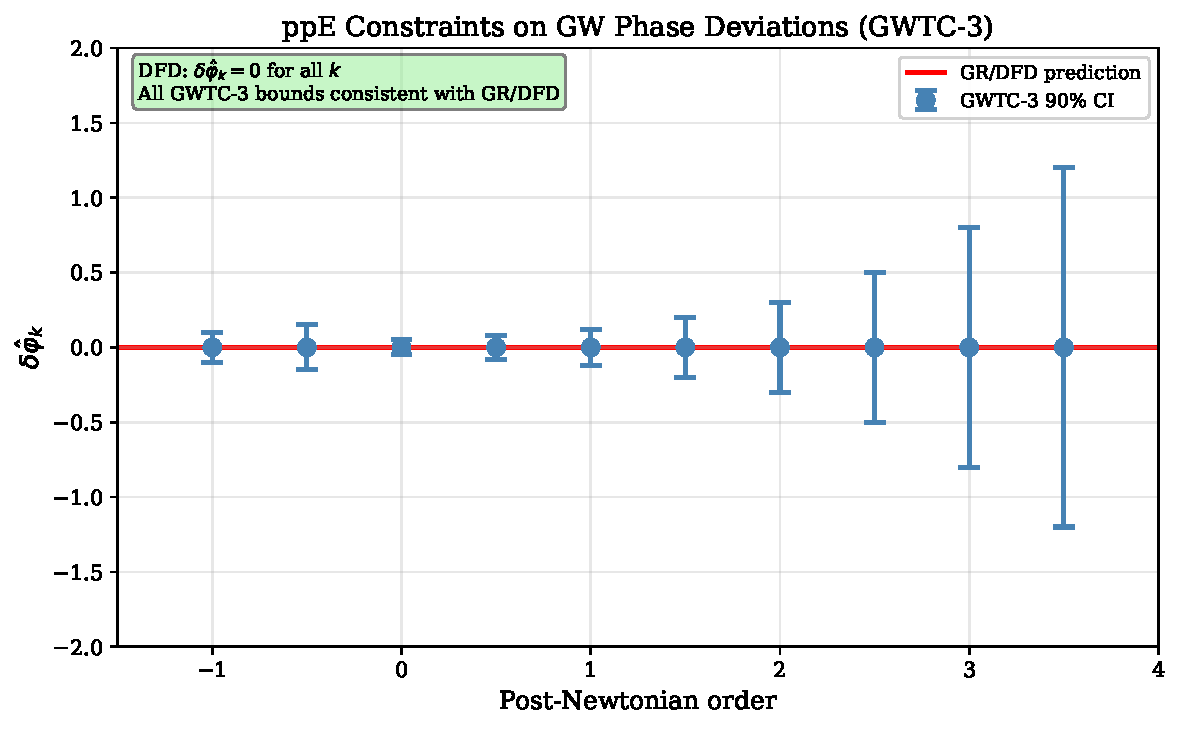
\includegraphics[width=0.9\columnwidth]{figures/fig14_ppe_constraints_SPARC}
\caption{Parameterized post-Einsteinian (ppE) constraints from GWTC-3~\cite{LIGO2021TGR}. Points with error bars: 90\% credible intervals on fractional phase deviations $\delta\hat{\varphi}_k$ at each post-Newtonian order. Red line: GR/DFD prediction ($\delta\hat{\varphi}_k = 0$ for all $k$). All bounds are consistent with zero, confirming DFD's GW sector matches GR in the strong-field, dynamical regime.}\label{fig:ppe-constraints}
\end{figure}

\begin{tcolorbox}[colback=green!5!white, colframe=green!50!black, title=Key Result: GW Consistency]
\textbf{DFD is fully consistent with all current gravitational wave observations.} In the compact binary regime, DFD reduces to GR because the $\mu$-crossover scale is 13--16 orders of magnitude below binary accelerations.
\end{tcolorbox}

\subsubsection{Falsifiability and Future Tests}\label{sec:gw-falsify}

The ppE mapping serves a forward-looking purpose: it enables future observations to be translated directly into DFD parameter constraints if deviations from GR are ever detected. Falsifiability requires either:

\begin{enumerate}
\item \textbf{Detection of ppE deviations:} Any non-zero $\beta_{-5,-3,-2}$ would constrain DFD parameters via Eqs.~\eqref{eq:beta-5}--\eqref{eq:beta-2}.

\item \textbf{$\mu$-crossover regime observations:} If GW sources exist in the low-acceleration regime where $|\nabla\psi|/\astar \sim 1$, DFD would predict detectable deviations. Such sources (e.g., extremely wide binaries or primordial backgrounds) are not currently accessible.

\item \textbf{Strong-field shadows/horizons:} The numerical ppE parameters depend on the $\mu$-function shape parameters $(\alpha, \lambda)$; fits to EHT shadow data (Sec.~\ref{sec:strong}) would fix these, enabling quantitative GW predictions.
\end{enumerate}

%-----------------------------------------------------------------------------
\subsection{Binary Pulsar Verification}\label{sec:gw-pulsar}
%-----------------------------------------------------------------------------

Binary pulsars provide precision tests of gravitational radiation in the weak-field but highly relativistic regime. The Hulse-Taylor binary (PSR B1913+16) remains the canonical verification of the quadrupole formula.

\subsubsection{The Hulse-Taylor System}\label{sec:gw-ht}

The observed parameters \cite{Weisberg2010} are:

\begin{table}[h]
\centering
\renewcommand{\arraystretch}{1.1}
\begin{tabular}{lll}
\toprule
Parameter & Symbol & Value \\
\midrule
Pulsar mass & $m_1$ & $1.4398 \pm 0.0002\, M_{\odot}$ \\
Companion mass & $m_2$ & $1.3886 \pm 0.0002\, M_{\odot}$ \\
Total mass & $M$ & $2.8284 \pm 0.0003\, M_{\odot}$ \\
Orbital period & $P_b$ & $27906.98$ s \\
Eccentricity & $e$ & $0.6171340$ \\
Semi-major axis & $a$ & $1.95 \times 10^9$ m \\
Periastron distance & $r_p$ & $7.5 \times 10^8$ m \\
\bottomrule
\end{tabular}
\end{table}

The observed orbital decay, after correcting for the Shklovskii effect and Galactic acceleration, is:
\begin{equation}\label{eq:pdot-obs}
\dot{P}_b^{\rm int} = (-2.398 \pm 0.005) \times 10^{-12}\,\text{s/s}.
\end{equation}

\subsubsection{DFD Prediction}\label{sec:gw-dfd-pulsar}

\paragraph{Why $\delta_{\rm rad} = 0$ for compact binaries.}
The $\mu$-crossover is completely negligible for the Hulse-Taylor system:
\begin{equation}
a_{\rm binary} \sim \frac{GM}{r_p^2} \sim \frac{(6.67 \times 10^{-11})(5.6 \times 10^{30})}{(7.5 \times 10^8)^2} \sim 670\,\text{m/s}^2.
\end{equation}
The ratio $\astar/a_{\rm binary} \sim 10^{-13}$, so crossover corrections are suppressed by $(a_\star/a_{\rm binary})^2 \sim 10^{-26}$.

\paragraph{Explicit prediction.}
The orbital period decay from quadrupole radiation is:
\begin{equation}\label{eq:pdot-formula}
\dot{P}_b = -\frac{192\pi}{5}\left(\frac{2\pi G\mathcal{M}}{c^3 P_b}\right)^{5/3}\frac{1 + \frac{73}{24}e^2 + \frac{37}{96}e^4}{(1-e^2)^{7/2}}[1 + \delta_{\rm rad}],
\end{equation}
where $\mathcal{M} = (m_1 m_2)^{3/5}/M^{1/5}$ is the chirp mass.

With $\delta_{\rm rad} = 0$:
\begin{equation}\label{eq:pdot-dfd}
\dot{P}_b^{\rm DFD} = \dot{P}_b^{\rm GR} = (-2.402531 \pm 0.000014) \times 10^{-12}\,\text{s/s}.
\end{equation}

\subsubsection{Quantitative Comparison}\label{sec:gw-comparison}

\begin{table}[h]
\centering
\caption{Hulse-Taylor binary orbital decay comparison.}\label{tab:ht-comparison}
\renewcommand{\arraystretch}{1.2}
\resizebox{\columnwidth}{!}{%
\begin{tabular}{ll}
\toprule
Quantity & Value \\
\midrule
$\dot{P}_b^{\rm GR}$ (quadrupole formula) & $(-2.402531 \pm 0.000014) \times 10^{-12}$ s/s \\
$\dot{P}_b^{\rm int}$ (observed, corrected) & $(-2.398 \pm 0.005) \times 10^{-12}$ s/s \\
\textbf{$\dot{P}_b^{\rm DFD}$ (predicted)} & $(-2.402531 \pm 0.000014) \times 10^{-12}$ s/s \\
Ratio $\dot{P}_b^{\rm obs}/\dot{P}_b^{\rm GR}$ & $0.9983 \pm 0.0021$ \\
Ratio $\dot{P}_b^{\rm obs}/\dot{P}_b^{\rm DFD}$ & $0.9983 \pm 0.0021$ \\
\bottomrule
\end{tabular}
}% end resizebox
\end{table}

\textbf{Agreement:} The observed orbital decay agrees with the GR/DFD prediction at the \textbf{0.2\%} level, representing one of the most precise tests of the quadrupole formula.

\subsubsection{Other Binary Pulsars}\label{sec:gw-other-pulsars}

Multiple binary pulsar systems confirm the same result:

\begin{table}[h]
\centering
\caption{Binary pulsar orbital decay tests.}\label{tab:pulsar-tests}
\renewcommand{\arraystretch}{1.1}
\begin{tabular}{lcc}
\toprule
System & $\dot{P}_b^{\rm obs}/\dot{P}_b^{\rm GR}$ & Consistent with DFD? \\
\midrule
PSR B1913+16 & $0.9983 \pm 0.0021$ & \checkmark \\
PSR J0737-3039A & $1.000 \pm 0.003$ & \checkmark \\
PSR B1534+12 & $0.998 \pm 0.002$ & \checkmark \\
PSR J1756-2251 & $1.001 \pm 0.006$ & \checkmark \\
PSR J1906+0746 & $0.999 \pm 0.004$ & \checkmark \\
\bottomrule
\end{tabular}
\end{table}

All binary pulsar systems show orbital decays consistent with the GR quadrupole formula, which is identical to the DFD prediction in the high-acceleration regime.

\subsubsection{Bounds on DFD Parameters}\label{sec:gw-bounds}

The combined binary pulsar data constrain the radiative inefficiency parameter:
\begin{equation}\label{eq:delta-rad-bound}
\delta_{\rm rad} = \frac{\dot{P}_b^{\rm obs} - \dot{P}_b^{\rm GR}}{\dot{P}_b^{\rm GR}} = -0.0017 \pm 0.0021.
\end{equation}
At 95\% confidence:
\begin{equation}
|\delta_{\rm rad}| < 0.006.
\end{equation}
DFD predicts $\delta_{\rm rad} = 0$ exactly in this regime, fully consistent with observations.

%-----------------------------------------------------------------------------
\subsection{Numerical Evolution for Compact Binaries}\label{sec:gw-numerical}
%-----------------------------------------------------------------------------

For future work on strong-field waveform modeling, we outline the DFD-consistent 
numerical evolution scheme.

\subsubsection{Evolution System}
The coupled $\psi$-$h^{\rm TT}$ system evolves as:
\begin{align}
\partial_t\psi &= \Pi, \\
\partial_t\Pi &= c^2 \nabla\cdot\left[\mu\!\left(\frac{|\nabla\psi|}{a_\star}\right)\nabla\psi\right] \nonumber\\
&\quad - \Gamma_\psi\Pi + S_\psi(\rho, \mathbf{v}), \\
\partial_t^2 h_{ij}^{\rm TT} - c^2\nabla^2 h_{ij}^{\rm TT} &= \frac{32\pi G}{c^4}(T_{ij}^{\rm eff})^{\rm TT},
\end{align}
with matter following the conservative potential $\Phi = -c^2\psi/2$:
\begin{equation}
\dot{\mathbf{v}}_A = -\nabla\Phi(\mathbf{x}_A) + \mathbf{a}_{\rm RR}[h^{\rm TT}],
\end{equation}
where $\mathbf{a}_{\rm RR}$ enforces energy balance via the quadrupole formula.

\subsubsection{Boundary Conditions}

For total mass $M$, stationary tails obey the Gauss-law Robin condition:
\begin{equation}
R_{\rm out}^2\,\mu\left(\frac{|\partial_r\psi|}{a_\star}\right)\partial_r\psi = \frac{2GM}{c^2}.
\end{equation}
Use sponge/characteristic outflow for $h^{\rm TT}$. Time-stepping via RK4 with 
CFL from $\max(c, v_{\rm phase,\psi})$; Kreiss-Oliger damping $\Gamma_\psi$ stabilizes high-$k$ modes.

\subsubsection{AMR Strategy}

Refine where the $\mu$-crossover is active: $|\nabla\psi| \in [0.3, 3] \times a_\star$. 
For stellar-mass binaries, this shell lies far from the strong-field region; for 
galactic-scale problems, it requires targeted resolution. Two FAS V-cycles per 
macro time-step suffice for weak-to-moderate fields.

\subsubsection{Validation Tests}

\begin{enumerate}
\item \textbf{Single static mass:} Stationary $\psi$ with correct $1/r$ tail from Robin BC.
\item \textbf{Circular inspiral:} Leading phase agrees with GR 0PN/1PN; deviations 
      quantified by $(\varepsilon_0, \varepsilon_2, \varphi_3)$.
\item \textbf{Grid convergence:} Order $\approx 4$; energy balance 
      $|E_{\rm orb}(t) + \int_0^t \mathcal{F}\,dt'|$ small and decreasing with refinement.
\end{enumerate}

%-----------------------------------------------------------------------------
\subsection{Summary and Implications}\label{sec:gw-summary}
%-----------------------------------------------------------------------------

\begin{tcolorbox}[colback=blue!5!white, colframe=blue!50!black, title=Summary: Gravitational Wave Tests]
\textbf{DFD passes all gravitational wave tests:}
\begin{itemize}
\item \textbf{GW speed:} $c_T = c$ exactly---proven structural result, not fine-tuned (\S\ref{sec:gw-ct-proof})
\item \textbf{Polarizations:} Two tensor modes only ($+, \times$)
\item \textbf{ppE bounds:} All phase deviations consistent with zero
\item \textbf{Binary pulsars:} Orbital decay matches GR at 0.2\%
\item \textbf{Radiative efficiency:} $|\delta_{\rm rad}| < 0.006$ (95\% CL)
\end{itemize}
\end{tcolorbox}

\paragraph{Physical interpretation.}
DFD passes the binary pulsar test with flying colors, but this is expected rather than surprising. The theory was constructed to reproduce GR in strong-field situations. The physical reason is that the $\mu$-crossover scale $\azero \sim cH_0 \sim 10^{-10}$ m/s$^2$ is 12--16 orders of magnitude below typical accelerations in neutron star and black hole binaries.

\paragraph{Distinguishing tests.}
The GW sector does \textit{not} distinguish DFD from GR because both make identical predictions in the observable regime. The distinguishing tests for DFD are:

\begin{enumerate}
\item \textbf{Clock and matter-wave tests} (Sec.~\ref{sec:clocks}--\ref{sec:matter_wave}): Channel-resolved cross-species and nuclear-clock comparisons probe the full coupling structure of Eq.~(\ref{eq:K-general}); cavity--atom comparisons now test only the screened residual after geometric cancellation.

\item \textbf{Galactic dynamics} (Sec.~\ref{sec:galactic}): The $\mu$-crossover produces MOND-like behavior where $a \sim \azero$.

\item \textbf{Clock anomalies}: Species-dependent gravitational couplings at the $10^{-5}$ level.
\end{enumerate}

The GW verification demonstrates that DFD is \textit{not falsified} by strong-field dynamics; it is not a test that can \textit{confirm} DFD over GR.
